\documentclass[10pt]{article}
\usepackage[a4paper,margin=17mm]{geometry}
\usepackage{graphicx,hyperref,booktabs,amsmath}
\hypersetup{colorlinks=true,urlcolor=blue}
\sloppy
\setlength{\parindent}{0pt}\setlength{\parskip}{5pt}
\begin{document}
\begin{center}\Large Bounded quadratic-monomial cancellation\\[3pt]
\normalsize Checked polynomial units; unchanged curve search --- 17 November 2026\end{center}
The Rust module cancels degree-two monomial columns using constant-weight
combinations of original rows. It solves new coupled-quadratic polynomial
controls over Fp29 and the Curve25519 prime. On 28 curve controls, outcomes and
node counts remain unchanged. Core PCC-20261117-1ab7fd; literature 3187dc;
separate runtime contract 6a68d9. All unsigned/unverified. [pcc:unverified]

\begin{center}\begin{tabular}{lrrr}\toprule
Same 28 curve inputs & Root & Unsupported & Model cap\\\midrule
Old v1 / exact Off &15&13&0\\
Bounded monomial v1 &15&13&0\\\bottomrule
\end{tabular}\end{center}
Fixed preservation and polynomial-cancellation gates pass; completed-curve
pruning is not observed at this implementation/domain. This does not reject
all linearization, other solvers or index calculus. [pcc:unverified]

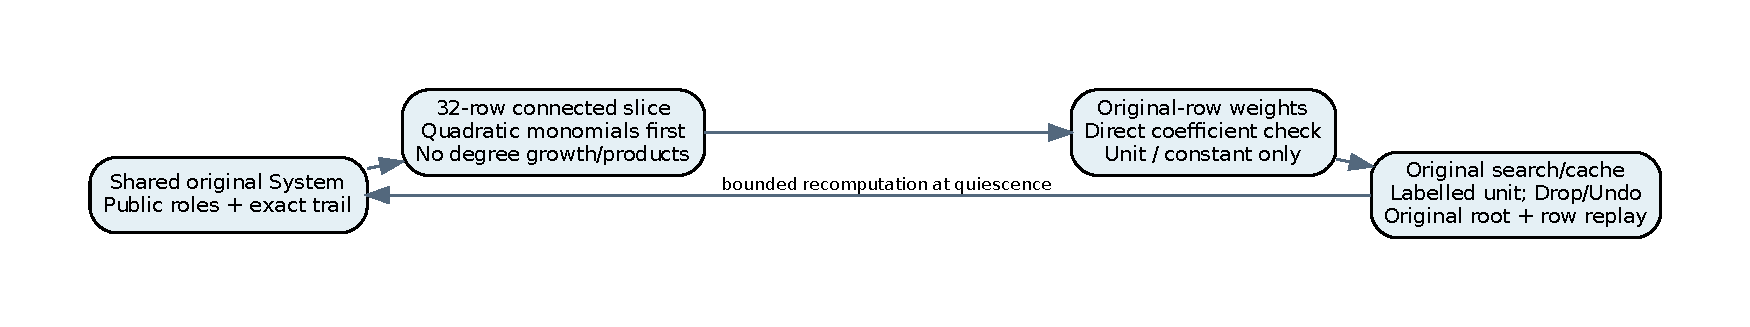
\includegraphics[width=\linewidth,height=34mm,keepaspectratio]{pipeline.pdf}\par
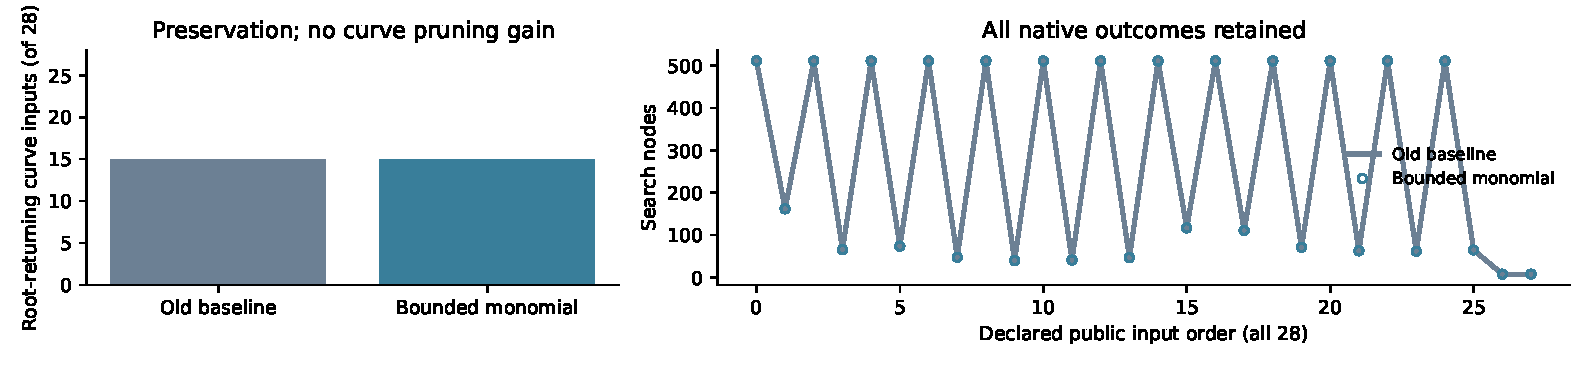
\includegraphics[width=\linewidth]{outcomes.pdf}\par
Native recorded values only, all 28 curve outcomes retained. No timing,
statistical fit or scaling inference. Caps and Unsupported are not absence
certificates. [pcc:unverified]

\textbf{Construction.} Share original System, dependencies and cache. A greedy
connected slice retains at most32 rows, 64 original unknown variables and 256 input
coefficient entries. Pivot quadratic columns before linear; constant stays augmented.
Carry original-row weights and admit only a checked linear unit/nonzero
constant, with exact premises and labelled unit applications. Drop leases
before LIFO Undo. No row products, degree growth or monomial multipliers;
composed univariate quadratics are discarded. This is incomplete classical
degree-two linearization, not full XL/F4 or a Gr\"obner basis. [pcc:unverified]

\textbf{Controls and interface.} Core 35 unique systems retain old 33 plus two
polynomial controls. Old and Off match full answers, decisions, counters and schedule.
All returned curve roots receive original-equation and indexed-row/group
replay. Only public System/roles/mode/limits enter solve; witness, scalar, signs,
labels, point lists and replay tables do not. [pcc:unverified]

\textbf{Domains.} Toy $p=101$, $A=95$, $h=(17,12)$, $a=17$, $q=3$, $k=8$, arity two, 13 image targets,
aliases retained, identity columns excluded. Actual curve $p=2^{255}-19$,
$A=486662$, $h_{new}=h_{old}^{213156431}$, $a=60824497$, $q=1$, $k=2$, arity two, TWO columns.
Huge originalq213156431 systems receive zero solver calls. [pcc:unverified]

\newpage
\begin{center}\Large Runtime contract, custody and next gate\end{center}
\textbf{Polynomial controls.} Public $xy+x-1=0$, $xy+2x-3=0$ exposes a
checked unit. Both Fp29 and $p=2^{255}-19$ produce a root in 1 node where old
extraction is Unsupported in 1 node. These are not curve decompositions.
Core synthetic rollback now finishes at root (3 to 1 nodes). Its AUTHORED
lease-reader fixture has placeholder counters, not measured engine behavior.
All 10 core trace/root/unit corruptions, 8 forced caps and 4 malformed refusals
remain. [pcc:unverified]

\textbf{Separate actual-engine contract.} Fp29 equations $z^2-z=0$,
$zu+u+v-1=0$, $zv+u+v-2=0$, branch role $z$. Old extraction is Unsupported
after 3 nodes; new engine returns $(1,0,1)$ in 3 nodes with 2 activations, 2 Drops,
1 Undo. Full 24,389 original assignments have 1 root; full reader accepts, while
missing-Drop/wrong-Undo refuse. This separate one-system correctness round
closes runtime coverage without editing/rerunning core 35. [pcc:unverified]

\textbf{Accounting stays open.} Caps remain1024 nodes, depth 128, 10 million
diagnostic events and 64 MiB CUMULATIVE MODELED reservations, 4096 variables,
8192 equations, 32768 terms and degree two; extra 1024-pass and 65536-event trace guards and fixed slice remain.
New arithmetic, scans, weights, checker work and modeled reservations are charged. Whole
cold parsing, serialization, replay, allocator and container overhead, and live storage costs remain
unpriced. No timing, speedup, complete-cost or exponent result. [pcc:unverified]

\textbf{Frozen core.} Composite 140 inputs: old 133 plus 7 new Cargo/Rust files; exact 28 old
request bytes reused,7 archive round-trips and 36 compiled bindings matched.
New 16508-byte source delta SHA-256:\\
\texttt{debfd1a9bac20a2899ee329f6f56685b6f88eee0a19be7910348dafe2f3a4abb}.\par
Copied 3375440-byte executable SHA-256:\\
\texttt{7c3f639c461a4cfaa7d480f0e26d044708f2246357e36d274e3737b84fa4c6b5}.\par
Raw 262 files / 9294358 bytes, 36380-byte archive SHA-256:\\
\texttt{ce91078fa0379457663df2d2454e94b25fa0b6b459b960b9f24da71600c62d14}.\par
Separate runtime context 143: core 140 plus 3 helper inputs, 4396-byte source delta.
Copied 1163056-byte executable SHA-256:\\
\texttt{a33cf3b2053489e8632f8a094f5d39a64fbc9fb20dae8db63c915f84a4c13625}.\par
Raw 8 files / 36567 bytes, 2020-byte archive SHA-256:\\
\texttt{2bbb7a93b2d338dffa88e69f670bd49fd3c7f42b1f8345ebff2a11eebd67f1a5}.\par
No monolithic 140- or 143-input archive. Distinct copied qualifiers and build/pre/post
records precede calls. Native results aggregate in Rust. Core first release
library controls, fmt, strict Clippy, build and helper checks pass; no source correction
or cap tuning. Initial sparse-archive metadata refusal preceded any qualified
call; exact tracked blobs restored, existing new bytes retained. [pcc:unverified]

\textbf{Prior art and next hypothesis.} Courtois/Klimov/Patarin/Shamir,
author full text, section3 Definition3.01 and appendix8:
\url{https://www.nicolascourtois.com/papers/xlfull.pdf}.
Linearization is classical; generic independence heuristics are not assumed.
KB absent/wrapper127; IACR conference/Diem full PDFs403, no Diem proof imported.
Next proposed successor admits certified univariate degree-at-most-two rows
with complete root-set/nonresidue checking and allowed public roles. Original
route-criteria V3 family, yield, selection, rank, kernel, recovery and cold-work gates
remain open. No successor campaign or performance-graph promotion.
[pcc:unverified]
\end{document}
